\chapter{Spectrometer Alignment} 
The alignment of the spectrometer is an important aspect for
reconstruction to ensure the track resolution is as accurate as
possible.  Without accurate alignment track reconstruction is not
possible and it is therefore not possible to analyze any data.  The
author of this prelim spent the summer of 2015 collecting alignment
data and was responsible for performing the alignment of the COMPASS
spectrometer.  There are over 200 tracking detector planes that need
to be aligned for four parameters: x position, y position, angle and
pitch.  The alignment procedure accomplishes this by minimizing a
$\chi^2$ function of all the track and detector parameters:
%
%\begin{dmath}
%  \chi^2 = \sum_{i=1}^{i=n_{tracks}}\sum_{j=1}^{j=n_{detectors}}
%  \frac{F_j(\alpha_t, \alpha_j)^2}{\sigma_j^2},
%  \label{equ:chi_align}%
%\end{dmath}
%
where $F_j(\alpha_t, \alpha_j)$ is the residual of each detector plane
and is a function of the track parameters, $\alpha_t$, and the
detector parameters, $\alpha_j$, and $\sigma_j$ is the position
resolution for detector $j$. The residual, $F_j(\alpha_t, \alpha_j)$,
is the difference between a detector hit location and the expexted hit
location based on a reconstructed track.  The track parameters,
$\alpha_t$, are the track x and y position at a specified detector and
the tangents $\frac{dx}{dz}$ and $\frac{dy}{dz}$ of the track momentum
at the same location.  These track parameters are different for each
track while the detector parameters, $\alpha_j$,
are the same for every track.  \par

Special low intensity muon beam, $\approx 10^5 \frac{\mu
  ^-}{\mathrm{spill}}$, data was taken each data period specifically
for alignment purposes.  A muon beam is desirable for alignment data
because the beam muons will interact less allowing for the alignment
procedure to assume straight tracks in the minimization problem.  At
the same time low intensity is chosen to reduce detector pile up
effects and make reconstruction in the central detector areas
possible.  For example to allow the beam killers on DC05 to be set to
nominal voltage.  As well the trigger system is modified to trigger on
beam and halo tracks which allow for a wider spread
beam to ensure the maximum illumination of the detectors.  \par

Two alignment runs with the previous beam settings were taken per data
period.  One run with the spectrometer magnets on and one with the
spectrometer magnets off.  The alignment run with magnets off was
performed as a first iteration to the alignment procedure.  The reason
for taking an additional alignment run with magnets on was because
some of the detectors close to the spectrometer magnets, particularly
those detectors close to SM1, would shift in the magnetic field and
therefore have different alignment locations with magnets on and
magnets off.  \par

To perform the $\chi^2$ minimization in the alignment procedure,
$F_j(\alpha_t, \alpha_d)$ is Taylor expanded and the partial
derivative of the $\chi^2$ function, equation~\ref{equ:chi_align}, is
taken with the respect to each track and alignment parameter and set
equal to zero.  The minimization process can be built into a matrix
equation where the size of the matrix to invert is
$(4n_{detector}+4n_{tracks})\times(4n_{detector}+4n_{tracks})$: \par
%
\begin{subequations}
  \begin{align}
    &F_j = F_j^0 + \sum_k \frac{\partial F_j}{\partial
      \alpha_k}\alpha_k \quad \text{Taylor expanding the residual for
      each detector plane.} \label{equ:F_taylor}\\ &\frac{1}{2}
    \frac{\partial \chi ^2}{\partial \alpha_i} = \sum
    _{t}^{n_{tracks}} \sum_j ^{n_{detectors}}\frac{1}{\sigma_j
      ^2}\frac{\partial F_j}{\partial \alpha_i}\Big ( F_j^0 + \sum_k
    \frac{\partial F_j}{\partial \alpha_k}\alpha_k \Big ) = 0 \quad
    \text{Minimizing the overall $\chi^2$.}\\ & \begin{bmatrix} \sum_j
      \frac{1}{\sigma^2_j}\frac{\partial F_j}{\partial
        \alpha_1}\frac{\partial F_j}{\partial \alpha_1} & \dots &
      \sum_j \frac{1}{\sigma^2_j}\frac{\partial F_j}{\partial
        \alpha_1}\frac{\partial F_j}{\partial \alpha_{4n_{tracks}}}
      \\ \vdots & \ddots & \vdots\\ \sum_j
      \frac{1}{\sigma^2_j}\frac{\partial F_j}{\partial
        \alpha_{4n_{tracks}}}\frac{\partial F_j}{\partial \alpha_1} &
      \dots & \sum_j \frac{1}{\sigma^2_j}\frac{\partial F_j}{\partial
        \alpha_{4n_{tracks}}}\frac{\partial F_j}{\partial
        \alpha_{4n_{tracks}}}
      \end{bmatrix}
    \begin{bmatrix}
      \alpha_1 \\ \vdots \\ \alpha_{4n_{tracks}}
    \end{bmatrix}
    = -
    \begin{bmatrix}
      \sum_j \frac{1}{\sigma^2_j}\frac{\partial F_j}{\partial
        \alpha_1} F_j^0 \\ \vdots \\ \sum_j
      \frac{1}{\sigma^2_j}\frac{\partial F_j}{\partial
        \alpha_{4n_{tracks}}} F_j^0 \\
    \end{bmatrix} \label{equ:aliMatrix}
  \end{align}
  \label{equ:Alignment}
\end{subequations}
%    %\text{Resulting equation to be solved.}
A normal alignment run results in over 200,000 tracks meaning the
matrix equation in equation~\ref{equ:aliMatrix} is huge and infeasible
to solve.  Fortunately many of the entries in the matrix are zero and
it can be shown that this matrix inversion can be reduced to the
inversion of several smaller matrices~\cite{matrix_inv}.  \par

%\begin{figure}[h]
%  \centering
%  \begin{subfigure}[t]{0.3\textwidth}
%    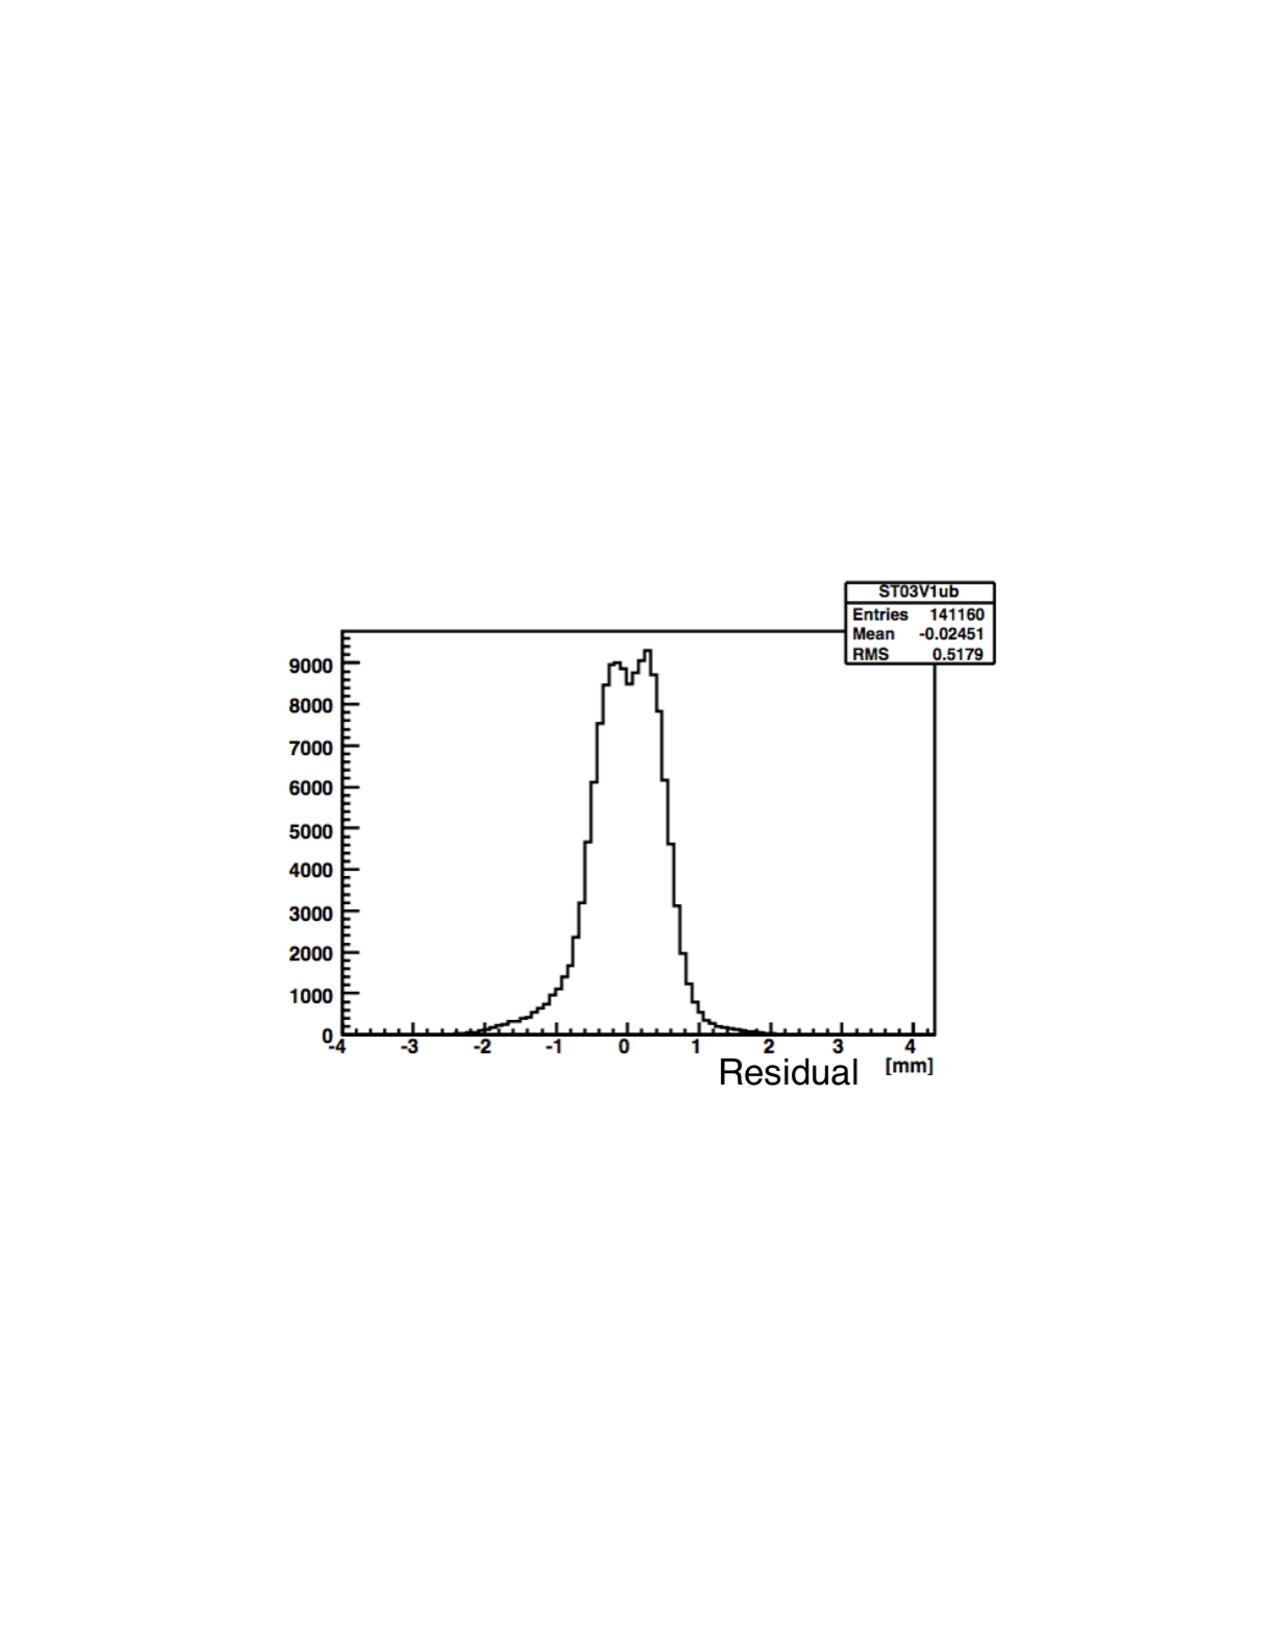
\includegraphics[width=\textwidth]{PositionResidual}
%    \caption{This plot tells if the detector is shifted in position or
%      not.}
%    \label{fig:PosRes}%
%  \end{subfigure}
%  \begin{subfigure}[t]{0.3\textwidth}
%    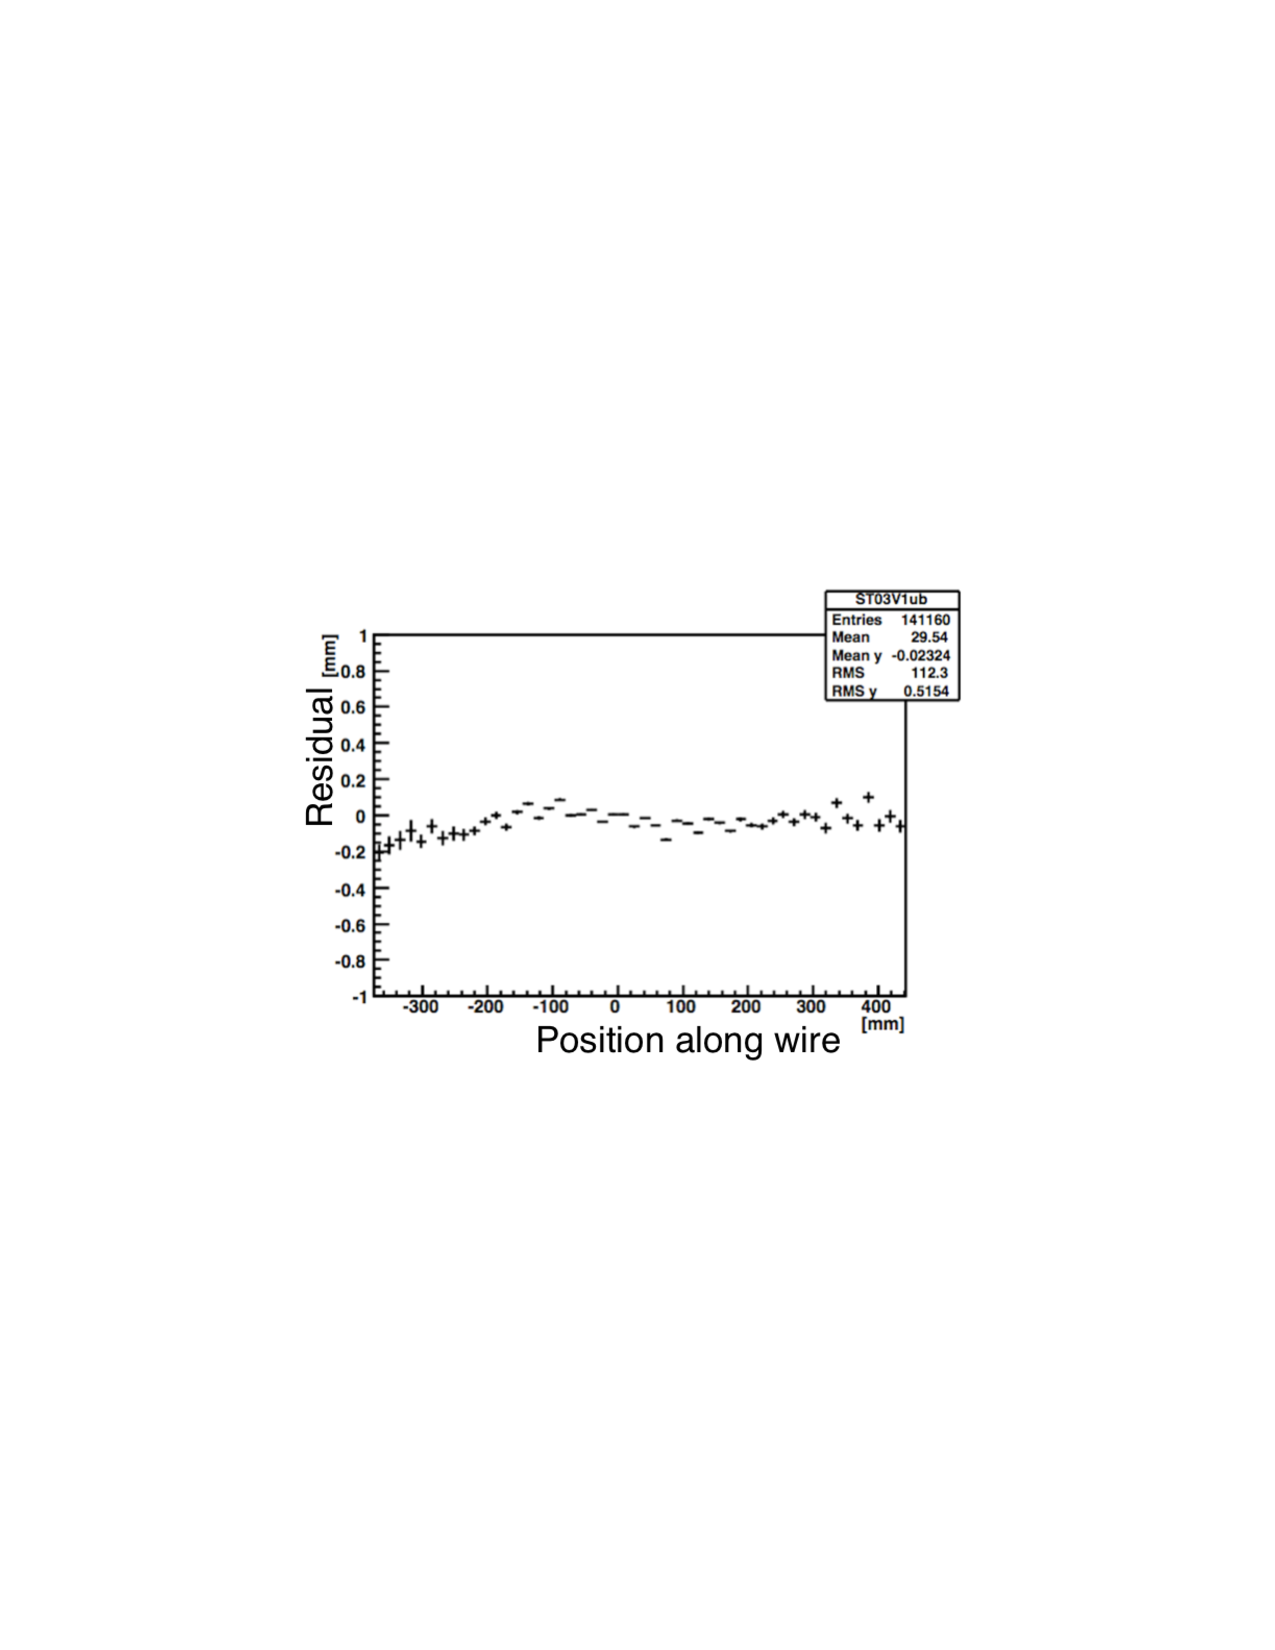
\includegraphics[width=\textwidth]{AngleResidual}
%    \caption{This plot is used to determine if the detector has the
%      correct angle.}
%    \label{fig:AngRes}%
%  \end{subfigure}
%  \begin{subfigure}[t]{0.3\textwidth}
%    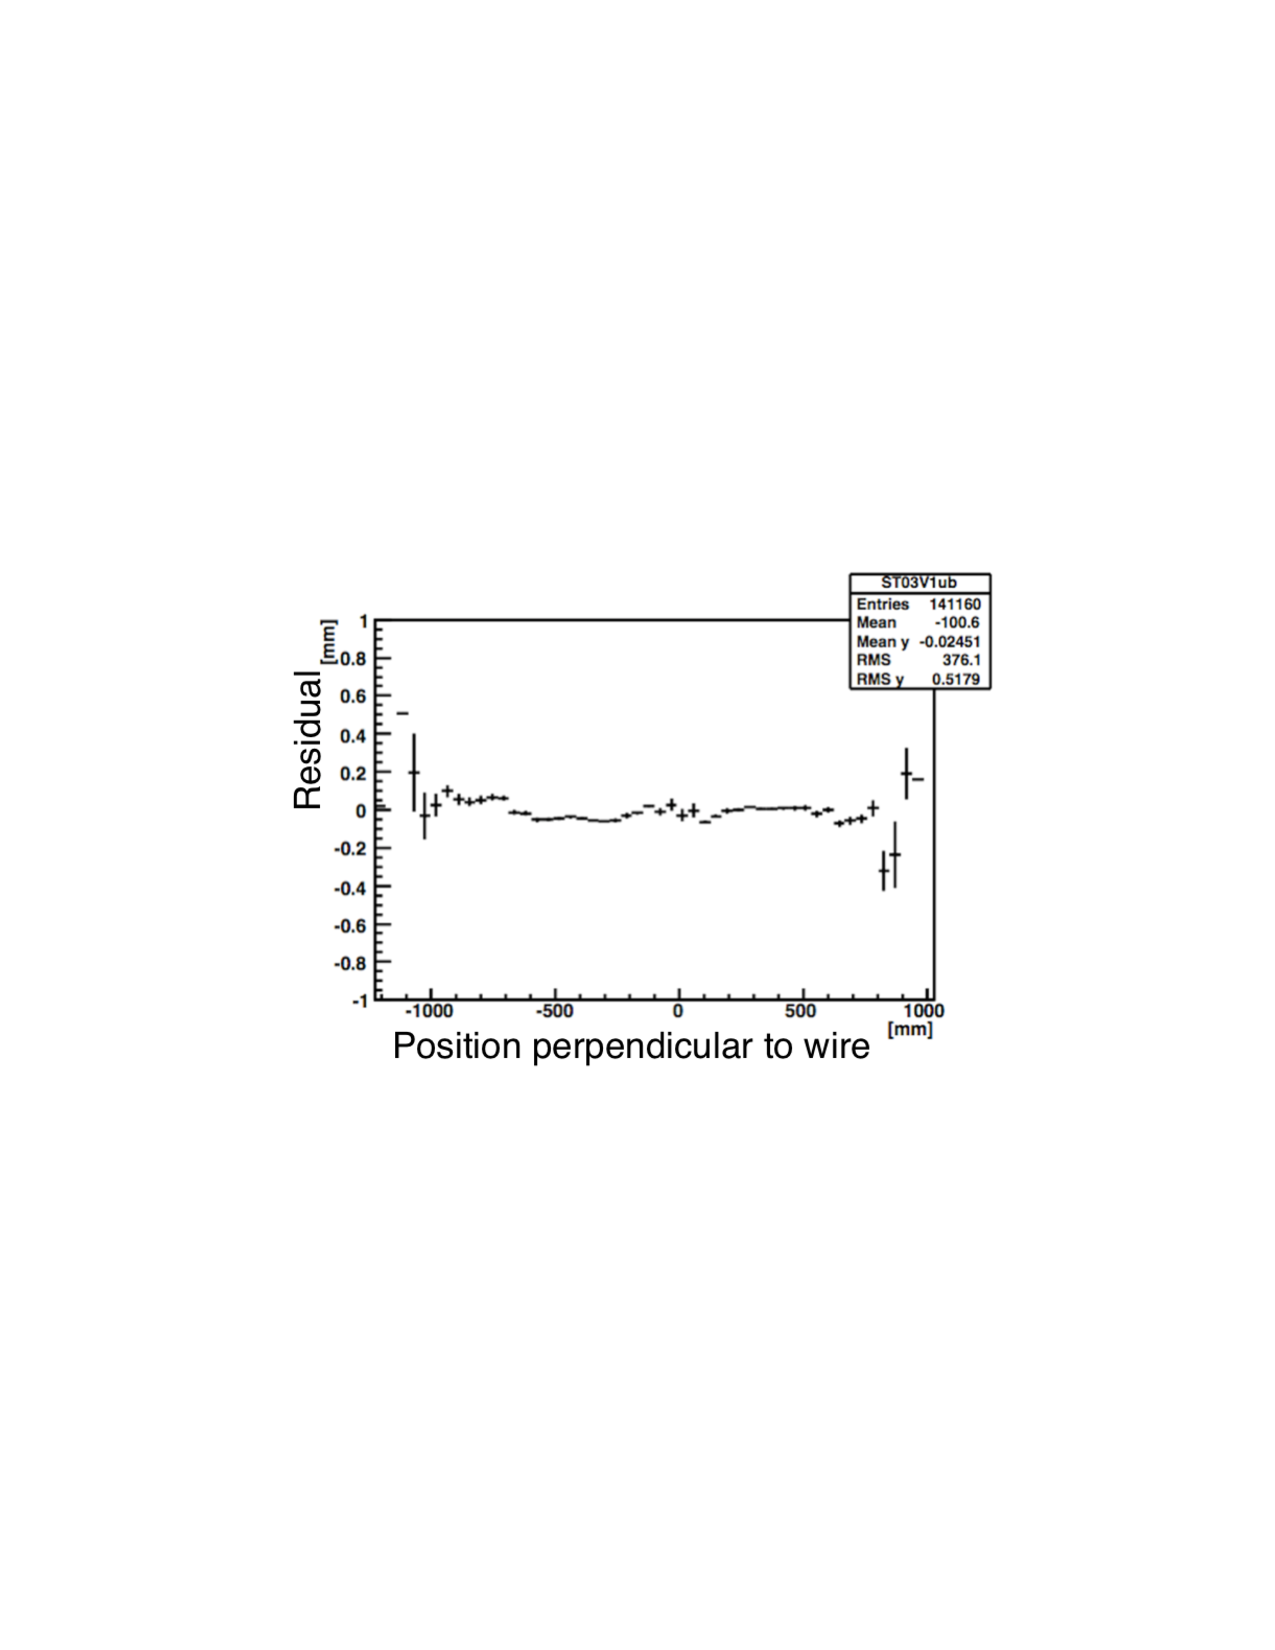
\includegraphics[width=\textwidth]{PitchResidual} 
%    \caption{This plot is used to determine if the detector wires have
%      the correct pitch.}
%    \label{fig:PitchRes}%
%  \end{subfigure}
%  \caption{Different residual distributions for a plane of a straw
%    detector at COMPASS.}
%  \label{fig:AlignRes}
%\end{figure}

In each iteration of the alignment procedure the matrix inversion in
equation~\ref{equ:aliMatrix} is performed.  All alignment tracks are
reconstructed based off the starting positions of all the detectors
and after each iteration the detector parameters are updated to reduce
the overall $\chi^2$ value.  Several iterations of the alignment
procedure are therefore required and are performed to ensure the
procedure converges.\par

The final product of the alignment procedure is an alignment file, for
each data period, that describes the location of every detector and is
used in all the data analysis.  For quality assurance several residual
distributions are plotted after each iteration for all the detectors.
The overall residual distribution is used to tell if a detector is
shifted, the change in residual as a function of the distance parallel
to the wires tells if a detector is rotated and the change in residual
as a function of the distance perpendicular to the wires tells if a
detector has been assigned the correct wire pitch in the alignment
file.  Examples of these residuals, to check are shown in
figure~\ref{fig:AlignRes}.


